\section{Прямое произведение групп. Свойства прямого произведения групп.}

\begin{defn}
  Прямым произведением групп $ G_{1}, G_{2} $ назовём \newline
  $ G_{1} \times G_{2} = \{ (g_{1}, g_{2}) | g_{1} \in G_{1}, g_{2} \in G_{2} \} $
\end{defn}

Введем произведение на $ G_{1} \times G_{2} $: \newline 
$ (g_{1}, g_{2}), (w_{1}, w_{2}) \in G_{1} \times G_{2}; (g_{1}, g_{2})(w_{1}, w_{2}) = (g_{1}w_{1}, g_{2}w_{2}) $

\begin{thm}
  $ G_{1} \times G_{2} $ - группа.
\end{thm} 

Естественным образом определяются проекции на сомножители \newline 
$ h_{1}(g_{1},g_{2}) = g_{1}, \, ker \, h_{1} = \{ (e_{1}, g) \; | \; g \in G_{2} \} \overset\sim{=} G_{2} $ \newline
$ h_{2}(g_{1},g_{2}) = g_{2}, \, ker \, h_{2} = \{ (g, e_{2}) \; | \; g \in G_{1} \} \overset\sim{=} G_{1} $ \newline \newline
Из основной теоремы о гомоморфизме следует также \newline
$ (G_{1} \times G_{2})/G_{2} = G_{1}, (G_{1} \times G_{2})/G_{1} = G_{2} $

\begin{thm}[Категорное свойство прямого произведения]
  $ M = G_{1} \times G_{2} $, $ W $ - некоторая группа. \newline
  $  \exists ! \phi $ - гомоморфизм, делающий диаграмму коммутативной. \newline
  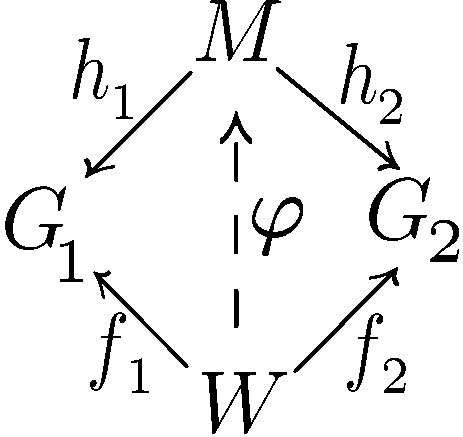
\includegraphics[scale = 0.3]{question9_1.pdf}
\end{thm}

\begin{thm}
  Приведенное выше свойство может быть принято за определение прямого произведения с точностью до изоморфизма.
\end{thm}



